\chapter[Lezione IX]{Lezione IX\newline\small{\emph{19/05/2011}}}
	\section{Rappresentazione dei numeri nel calcolatore}
Un sistema di rappresentazione numerica può essere \emph{posizionale} o \emph{non posizionale}. Nel primo caso, ogni cifra assume un peso diverso a seconda della posizione in cui è scritta. Una rappresentazione numerica è anche caratterizzata dalla \emph{base}, che fissa il numero massimo di simboli differenti che consentiti per rappresentare le cifre; il sistema numerico occidentale è \emph{decimale posizionale}. Pertanto:
\begin{itemize}
	\item
La base (\lstinline!10!) stabilisce il numero di simboli differenti consentiti per rappresentare le cifre (\lstinline!0, ... , 9!).
	\item
Il fatto che sia posizionale ci garantisce che, ad esempio, $123=1\cdot 10^2+2\cdot 10^1+3\cdot 10^0 \neq 321=3\cdot 10^2+2\cdot 10^1+1\cdot 10^0$. Ciò accade proprio perché le cifre hanno pesi differenti a seconda della loro posizione, infatti:
\[
4814=4\cdot10^3+8\cdot10^2+1\cdot10^1+4\cdot10^0.
\]
In generale, essendo $b$ la base della rappresentazione e $c_i$ (con $i\in\{1,\dots,b\}\cap\mathbb{N}$) i rappresentatori delle cifre, dato $z\in\mathbb{N}$  si ha che, $\forall i,\dots,j\in\Set{1,\dots,b}\cap\mathbb{N}$:
\[
c_{i_z}\dots c_{j_1}=c_{i_z}10^{z-1}+\dots+c_{j_1}10^{0}=\sum_{e=1}^z c_{\{i,\dots,j\}_e}\cdot b^{e-1}.
\]
\end{itemize}

		\subsection{Esempi}
		\label{subsec:BasiExamp}
Si considerino i seguenti esempi. Le basi \emph{ottale}, \emph{esadecimale} e \emph{binaria} non sono scelte a caso; esse, infatti, sono molto usate nel campo dell'informatica. Si noti che, nel caso di rappresentazioni non decimali, è buona norma specificare la base a pedice.
\begin{description}
\item[Base] \lstinline!8!
	\begin{itemize}
		\item
Simboli: \lstinline!0, 1, 2, 3, 4, 5, 6, 7!
		\item
$523_8=5\cdot8^2+2\cdot8^1+3\cdot8^0=339_{10}$
	\end{itemize}
\item[Base] \lstinline!16!
	\begin{itemize}
		\item
Simboli: \lstinline!0, 1, 2, 3, 4, 5, 6, 7, 8, 9, A, B, C, D, E, F!
		\item
$3A2_{16}=3\cdot16^2+A\cdot16^1+2\cdot16^0=930_{10}$
	\end{itemize}
\item[Base] \lstinline!2!
	\begin{itemize}
		\item
Simboli: \lstinline!0, 1!
		\item
$101101_{2}=1\cdot2^5+0\cdot2^4+1\cdot2^3+1\cdot2^2+0\cdot2^1+1\cdot2^0=45_{10}$
	\end{itemize}
\end{description}

		\subsection{Passare in base \lstinline!2!}
Per passare da una base, ad esempio \lstinline!10!, in base \lstinline!2!, si può utilizzare il seguente metodo\footnote{Si noti che per passare ad una base $b$ qualsiasi, si può usare lo stesso procedimento sostituendo a \lstinline!2! il numero $b$.}, che è il procedimento inverso di quelli mostrati nel paragrafo~\vref{subsec:BasiExamp}.

S'individua la massima potenza di \lstinline!2! che non supera il numero $m$ di partenza (sia essa $n$). Se $2^n-m=z_1=0$, il numero binario si ottiene ponendo $1$ nella posizione $n+1$ e zero nelle posizioni da $n$ in giù. In caso contrario ($z_1\neq0$), si trova la massima potenza di \lstinline!2! che non superi $z_1$ e si ripete il procedimento finché non s'individua un indice $i\in\{1,\dots,\log_2n+1\}\cap\mathbb{N} \mid z_{i}=0$. Ad esempio:
\[
45_{10}=\underbrace{32+8+4+1}_{2^5+2^3+2^2+2^0}=101101_{2}
\]

Tale algoritmo, tuttavia, è piuttosto scomodo da stendere come programma e risulterebbe ""pesante'' per il calcolatore. Si può allora pensare ad un altro procedimento.

Si divide il numero $m$ di partenza per \lstinline!2!. Il resto $r_1$ di tale operazione è la prima cifra (quella con il peso minore) del numero binario. Si divide ora il quoziente $q_1$ (intero) per \lstinline!2!. Come prima,  il resto è la seconda cifra del numero. Il procedimento termina quando s'individua un indice $i\in\{1,\dots,\log_2n+1\}\cap\mathbb{N} \mid q_{i}=0$. Ecco un esempio:
\[
\dfrac{45}{2}=22+\mathbf{1};\ 
\dfrac{22}{2}=11+\mathbf{0};\ 
\dfrac{11}{2}=5+\mathbf{1};\ 
\dfrac{5}{2}=2+\mathbf{1};\ 
\dfrac{2}{2}=1+\mathbf{0};\ 
\dfrac{1}{2}=0+\mathbf{1}.\ 
\]
Chiaramente, tale algoritmo è molto più semplice da tradurre in un programma in C e risulta molto più efficiente del precedente.

	\subsection{\lstinline!bit! e \lstinline!byte!}
L'unità di misura della memoria in un calcolatore è il \lstinline!bit! (\emph{Binary Digit}, cioè \emph{Cifra Binaria}). Il suo primo multiplo è il \lstinline!byte!\footnote{Corrispondente al ""quadretto'' nel paragrafo~\vref{sec:mem}} (\lstinline!1 byte = 8 bit!). Con un \lstinline!byte! si ottengono $2^8=256$ combinazioni differenti, quindi, in teoria, 256 caratteri diversi. In realtà, la combinazione \lstinline!00000000! non viene considerata un carattere, pertanto le rappresentazioni effettivamente ammesse sono $2^8-1=255$ (i caratteri ASCII). In generale, $n$ \lstinline!bit! danno $2^n$ combinazioni e $2^n-1$ rappresentazioni di caratteri.

Nel calcolatore, normalmente, una variabile di tipo \lstinline!int! occupa \lstinline!4 byte! ossia $(2^8)^4=2^{8\cdot4}=4294967296$ combinazioni. Se gli interi fossero soltanto positivi, il più grande numero rappresentabile sarebbe $4294967296-1=4294967295$. Tuttavia, variabili di tipo \lstinline!int! possono assumere valori sia positivi che negativi. Si stabilisce, allora, che il primo \lstinline!bit! di un intero sia destinato a contenere il segno del numero: per convenzione, \lstinline!0 = "-"! e \lstinline!1 = "+"!.

Si ammetta, per semplicità, che un intero sia rappresentato da \lstinline!4 bit!. Allora, le rappresentazioni \lstinline!1000! e \lstinline!0000! corrispondono ($-0_{10}=+0_{10}$). Avendo destinato un \lstinline!bit! al segno, restano soltanto $2^{\text{\em numero di \texttt{bit}}}-1$ rappresentazioni differenti, $255$ nella fattispecie. Per ovviare a questo problema, si ricorre al metodo del \emph{complemento a due}.

	\subsection{Complemento a due}

\begin{figure}
	\centering
	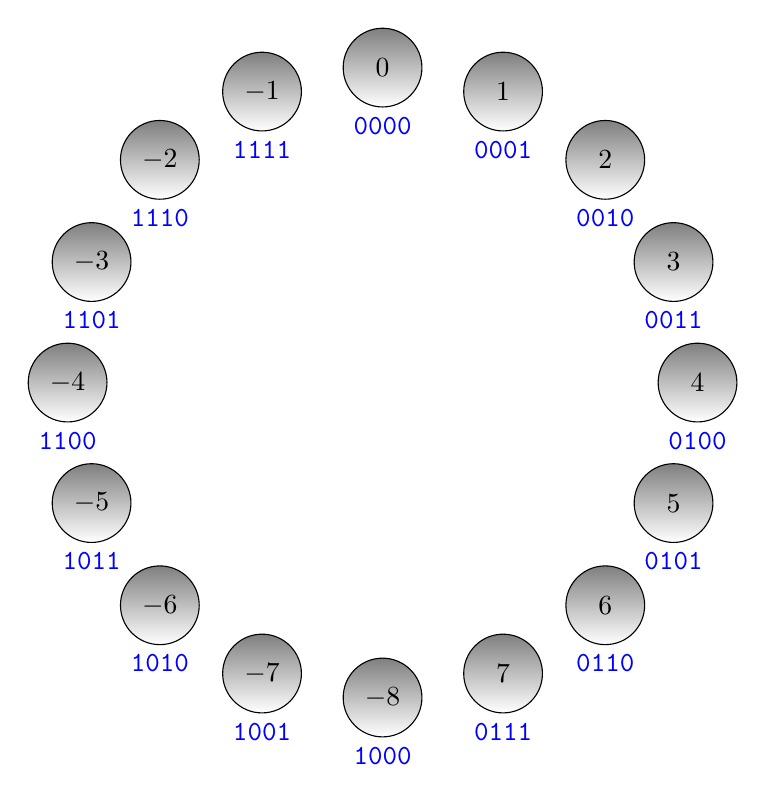
\begin{tikzpicture}[scale=0.8]
\foreach \ang/\dl/\bl in {90/0/0000,67.5/1/0001, 45/2/0010,
22.5/3/0011,0/4/0100,-22.5/5/0101,-45/6/0110,-67.5/7/0111,
-90/-8/1000,-112.5/-7/1001, -135/-6/1010,-157.5/-5/1011,
-180/-4/1100,-202.5/-3/1101,-225/-2/1110,-247.5/-1/1111} {
	\draw [black] node [circle,draw,minimum size=1cm,label=below:{\color{blue}$\mathtt{\bl}$},top color=gray] at (\ang:5) {$\dl$};
}
	\end{tikzpicture}
	\caption[Complemento a due]{Rappresentazione del complemento a due con numeri di \lstinline!4 bit!.}
	\label{fig:2comp}
\end{figure}

S'immagini di sistemare sul bordo di un anello tutte le combinazioni date da un certo numero di \lstinline!bit! (se ne considerino sempre \lstinline!4!, per comodità) come in figura \ref{fig:2comp}. Ora, s'interpretino nel modo usuale i numeri che hanno come prima cifra (partendo da sinistra) \lstinline!0!. Cominciando da \lstinline!0000! e spostandosi in senso orario, dunque, si hanno numeri interi crescenti fino al numero \lstinline!1000!. Si stabilisce, altresì, di assegnare ai numeri che hanno \lstinline!1! come prima cifra valori progressivamente più piccoli partendo da $-1$ (\lstinline!1111!) e proseguendo in senso antiorario.

Si ha che, ad esempio, considerando la somma delle rappresentazioni binarie dei numeri $-6_{10}$ e $-2_{10}$:
\[
	\begin{array}{r l}
\mathtt{1010}	&+	\\
\mathtt{1110}	&=	\\
		\midrule
\mathtt{11000}
	\end{array}
\]
Siccome un numero è composto di \lstinline!4 bit!, il calcolatore memorizzerà solo \lstinline!1000! che corrisponde a \lstinline!-8!. Si prendano altri casi:
\[
\mathtt{
3+(-5)=
	\begin{array}{r l}
\mathtt{0011}	&+	\\
\mathtt{1011}	&=	\\
		\midrule
\mathtt{1110}
	\end{array}
\quad \rightarrow-2_{10}
}
\]
Si noti che non c'è stato bisogno d'introdurre l'operazione di differenza. Una volta definita la somma, non serve altro. Ancora:
\[
\mathtt{
5+(-3)=
	\begin{array}{r l}
\mathtt{0101}	&+	\\
\mathtt{1011}	&=	\\
		\midrule
\mathtt{10010}
	\end{array}
\quad \rightarrow2_{10}
}
\]
Tuttavia:
\[
\mathtt{
3+6=
	\begin{array}{r l}
\mathtt{0111}	&+	\\
\mathtt{0110}	&=	\\
		\midrule
\mathtt{1101}
	\end{array}
\quad \rightarrow-3_{10}
}
\]
Ciò accade perché il numero \lstinline!13! non può essere rappresentato con \lstinline!4 bit!. Infatti, tale metodo è corretto solo per numeri $n\in\{-8,\dots,7\}\cap\mathbb{N}$ (o, in generale, essendo $m$ il numero di \lstinline!bit!: $-2^{m-1}-1\le n \le 2^{m-1}-1$). Questo è un errore comunemente chiamato \emph{overflow}.

		\subsection{Virgola mobile}
Finora, è stata trattata soltanto la rappresentazione di un intero ($n\in\mathbb{Z}$) in un calcolatore. Si considerino ora dei numeri $q\in\mathbb{Q}$. Affinché essi siano rappresentati in memoria si deve introdurre il concetto di \emph{virgola mobile} (o, in inglese, \emph{floating point}). Siano dati i seguenti numeri decimali:
\[
	\begin{split}
&2,718_{10}=2\cdot10^0+7\cdot10^{-1}+1\cdot10^{-2}+8\cdot10^{-3};	\\
&101,01_2=1\cdot2^2+0\cdot2^1+1\cdot2^0+0\cdot2^{-1}+1\cdot2^{-2}.
	\end{split}
\]
Nella sua rappresentazione più semplificata, un numero in virgola mobile è composto da:
\begin{itemize}
	\item
Mantissa;
	\item
Esponente;
	\item
Base.
\end{itemize}
Bisogna tenere conto che, come in precedenza, anche qui \lstinline!1 bit! viene riservato al il segno. Le cifre significative sono rappresentate dalla \emph{mantissa}. Si ha che:
\[
2,718_{10}=\underbrace{2718}_{\textit{Mantissa}}\cdot{\underbrace{10}_{\textit{Base}}}^{(-3)\ \rightarrow\textit{Esponente}}
\]
Tra le infinite rappresentazioni in virgola mobile, si stabilisce una forma ""canonica''. Essa prevede che:
\begin{itemize}
	\item
Siano $m, b$ rispettivamente la mantissa e la base, allora si deve avere che: $0<m<b$;
	\item
L'esponente della base dev'essere il più piccolo possibile.
\end{itemize}

In memoria, un numero in virgola mobile è rappresentato secondo il seguente schema:
\begin{center}
\textit{
	\begin{tabular}{|c|c|c|}
		\toprule
segno	&esponente	&mantissa	\\
		\bottomrule
	\end{tabular}
}
\end{center}


Se un numero in virgola mobile occupa \lstinline!32 bit!, a segno, esponente e mantissa vengono assegnati rispettivamente: \lstinline!1!, \lstinline!8! e \lstinline!23 bit!. Se ne occupa \lstinline!64!, invece: \lstinline!1!, \lstinline!11! e \lstinline!52 bit!.

Si tenga presente che nelle operazioni algebriche, il calcolatore interpreta la mantissa $m$ come se fosse $m+1$.

	\section{Strutture di controllo}
Durante \marginpar{Il ciclo \lstinline!for()!} tutta la trattazione è stata introdotta una sola notazione per le iterazioni: il ciclo \lstinline!while()! (vedi il paragrafo~\vref{sec:it}). Esiste, tuttavia, un altra sintassi che risulta in parecchie occasioni più conveniente: il ciclo \lstinline!for()!.
		\subsection{Ancora sulle iterazioni}
Il riquadro~\vref{cod:for()} mostra un ciclo \lstinline!while()! e il suo equivalente ciclo \lstinline!for()!. Il secondo prevede una sintassi molto più contenuta e, nella maggior parte dei casi, rende il codice molto più leggibile.



La sintassi del ciclo \lstinline!for! è:\\
\lstinline!for( /*istruzione 1*/; /*condizione*/; /*istruzione 2*/ )!.

Il compilatore:
\begin{itemize}
	\item
Esegue \lstinline!/*istruzione 1*/! (in genere, un assegnamento) una sola volta, all'inizio del ciclo;
	\item
Verifica la \lstinline!/*condizione*/!;
	\item
Se la \lstinline!/*condizione*/! è verificata, esegue il corpo del ciclo;
	\item
Esegue \lstinline!/*istruzione 2*/ !;
	\item
Verifica di nuovo la condizione; \\\vdots
\end{itemize}

\begin{code}
\centering
	\caption{Confronto tra il ciclo \lstinline!while()! ed il ciclo \lstinline!for()!.}
	\label{cod:for()}
\begin{minipage}{0.45\columnwidth}
	\begin{lstlisting}
int i = 0;
while ( i < N ) {
	s = s+p[i];
	i++;
}
	\end{lstlisting}
\end{minipage}	\hfill
\begin{minipage}{0.45\columnwidth}
	\begin{lstlisting}
int i;
for ( i = 0; i < 10; i++ ) {
	s = s+p[i];
}
	\end{lstlisting}
\end{minipage}
\end{code}